%!TEX root = ../report.tex

\begin{document}
	\let\cleardoublepage\clearpage
\chapter{Evaluation} \label{sec:evaluation}
In this section, we evaluate the proposed mediator architecture design based on whether it fulfills the requirements and solves the problem statement discussed in the section \ref{sec:problem_statement}. 

\section{Evaluation through requirements}
Context based data model - As we discussed in section \ref{sec:problem_statement}, in a multi-robot scenario the data generated by different robot sensors should be interpreted by other robots in the group. But the system in the robots might be developed by different developers and may use different attribute names. So there is a chance for misinterpretation of data during calculation also humans understand the context by seeing the data, but it is difficult for the machines. Our proposed system supports delivering contexts along with the response data. To achieve this, we created our own list of general vocab collection in terms of robot applications with all the meanings predefined in it. Also, the proposed data models relationship is improved over time to support secure data retrieval from the multi-databases with minimal effort through GraphQL queries.

\subsection{Generic query language}
Our mediator architecture is designed with GraphQL frameworks as a base, and the explanation for why we adopted this framework is discussed in section \ref{sec:graphql_falcor_conclusion}. GraphQL offers it's own query language to write/read data, and the learning curve is fast to understand this query language. So users/robots may use this generic query language to interact with datasources regardless of what type of database is running in the system.

\subsection{Type validation}
The current system is strongly bounded with types to avoid the problems or system failures during any necessary calculations in the robot to decide an action to perform. So the system doesn't allow to store any data with a type mismatch. 

\subsection{Scalability}
One can configure multiple databases with the current mediator with a single change in the mediator config file.

\subsection{Configurable data format support}
By default, the mediator system returns the response in JSON-LD format. But some legacy systems or the tool which consumes the data might need the response data in JSON or RDF format. In this case, consumers can directly transform JSON-LD data to other context based format such as RDF using external tools. However, one can set the response format in the mediator config and implement their logic for transformation in the mediator.

\subsection{Graphical User Interface}
Apollo GraphQL server is packed with an efficient GUI system to make queries or mutations on the database. This GUI system can be exposed over "/graphiql" endpoint on demand. This tool is beneficial for users to visually debug the sensor generated data or mock a dummy set of data in the database. Also, this tool offers schema introspection so that the users do not require to check the schema in the database whenever they query. 

\newpage

	\begin{figure}[H] 
		\begin{center}
			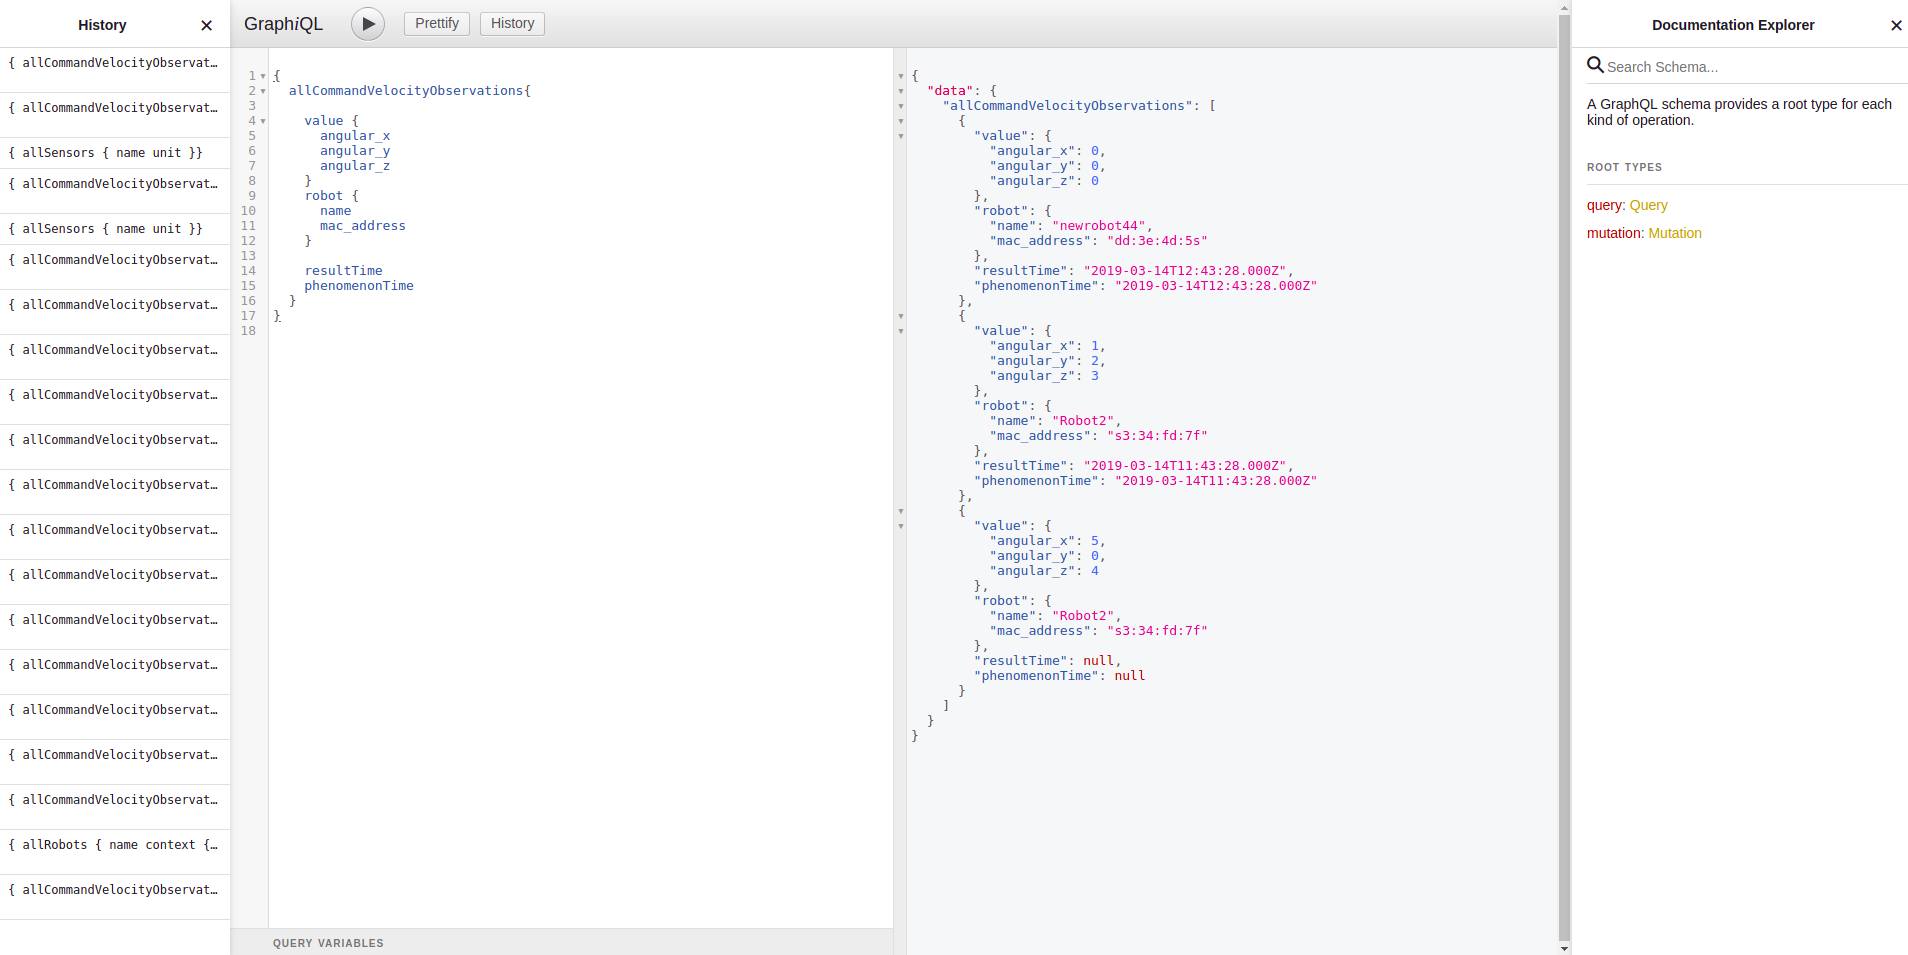
\includegraphics[scale=0.37,angle=90]{./images/png/graphiql_gui}	
			\caption{GraphiQL tool to mutate or query data visually from a browser}	
			\label{fig:graphiql_gui}	
		\end{center}
	\end{figure}
\thispagestyle{empty}

\newpage
Figure \ref{fig:graphiql_gui} shows the complete sections in the graphiql web-based user interface. There are four sections in the application. The first section shows a list of previously executed GraphQL queries, and it saves users time by not writing the same queries repeatedly. Next section gives space for the users to orchestrate GraphQL queries and it provides autocompletion feature to select the attributes under the specified data entity. The third section shows the result which is returned from GraphQL server. The last section provides an option for users to do introspection on schemas for queries and mutations.

\section{Evaluation against the existing system}
Existing black box system flattens the sensor generated data and stores them directly in its local MongoDB instance. And the problems in dumping the sensor data without proper modeling them is already discussed in section \ref{sec:problem_statement}. Also, the black box exposes a data query\_interface to apply filters and query data from the dump. However, the person who wants to debug the logs from multiple robots, they have to switch the database in the configuration before working on the query interface system. Our system design solves all these problems. For example, with the help of the current mediator system, one can configure multiple database instances and apply a single query to fetch data from all of them. Also, users can add filters and choose the data only from selected robots. The current system also provides a well-defined data model to connect specific task with robots and sensors which are involved in that task. In the end, by giving the JSON-LD context in the response solves the interoperability issue from existing black box system.
\end{document}
